\documentclass[sigconf]{acmart}
%%
%% \BibTeX command to typeset BibTeX logo in the docs
\AtBeginDocument{%
  \providecommand\BibTeX{{%
    \normalfont B\kern-0.5em{\scshape i\kern-0.25em b}\kern-0.8em\TeX}}}


\newcommand\myworries[1]{\textcolor{red}{#1}}

%%%%%%%%%%%%%%%%%%%%%%%%%%%%%%%%%%%%%%%%
% Inverting Colors to save my eye balls
%\usepackage{xcolor}
%\pagecolor[rgb]{0.1,0.12,0.15}
%\color[rgb]{.9,.9,.95}
%%%%%%%%%%%%%%%%%%%%%%%%%%%%%%%%%%%%%%%%

\citestyle{acmauthoryear}



\begin{document}

\title{Shape Matching Element Method}

%% A "teaser" image appears between the author and affiliation
%% information and the body of the document, and typically spans the
%% page.
\begin{teaserfigure}
  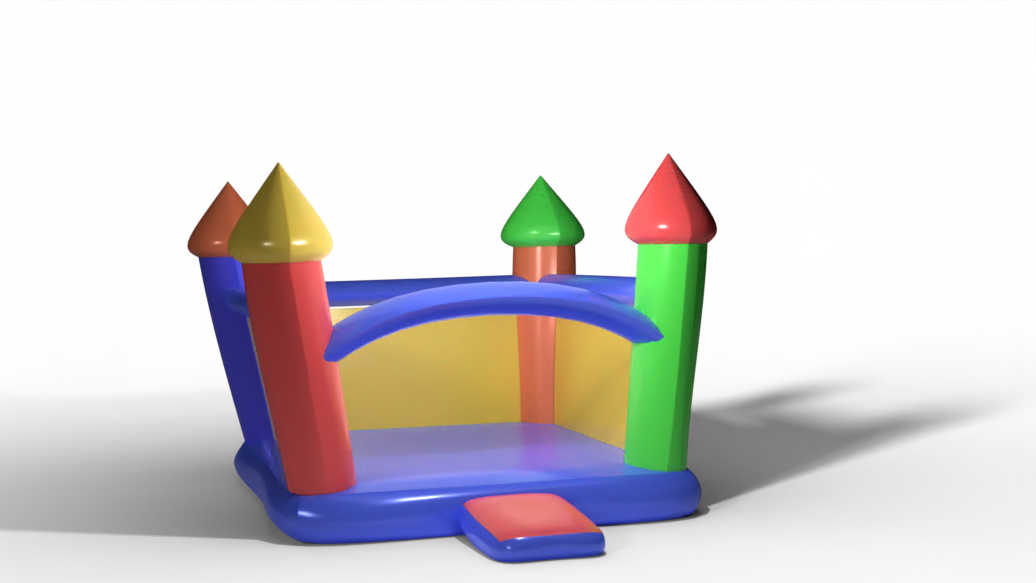
\includegraphics[width=\textwidth]{castle.png}
  \caption{tmp}
  \Description{}
  \label{fig:teaser}
\end{teaserfigure}

\maketitle

\section{Introduction}


% \textbf{x}(\textbf{X}) = \hat{A}M(\textbf{X}) + \bar{\textbf{x}}$ \\
% $\hat{A} = \sum_i^{|S|}w_i(\textbf{X})A_i$

We have $\mathbf{x} = (x_0, x_1)$ and $\mathbf{X} = (X_0, X_1) $ as deformed and undeformed positions, respectively. \\

\textbf{<insert Exposition about FEM >} \\
In our case, the function we are trying to evaluate is deformation with respect to the center of mass. In VEM, instead of reconstructing values of our function using nodal values, we seek to find a a set of polynomial coefficients that map some arbitrary undeformed position to a polynomial approximation of its deformed position. This set of polynomial coefficients is referred to as the projection operator, $\mathbf{\Pi}$. The key point here is that $\mathbf{\Pi}$ is constructed strictly using positions defined on the boundary, avoiding the need for explicit representation of the interior. \\

\subsection{Shape Matching: }
In shape matching, authors seek a polynomial transformation, $\mathbf{\Pi}$ that minimizes $\sum_i ||\mathbf{\Pi}\mathbf{M(X)} - \mathbf{p_i}||^2$ where $\mathbf{M(X)}$ is the monomial basis of the $i$-th boundary vertex and $\mathbf{p_i}$ is current displacement from the center of mass for the $i$-th point. We argue this paper can be interpreted as a sort of virtual element method. \\

\subsection{Reconstructing deformed positions}
A general form for the monomial basis takes the following form <insert here>. For example, in 2D with quadratic deformation we have:
\begin{equation}
    \mathbf{M(X)} =\begin{bmatrix}
    X_0 - \bar{X}_0  \\ 
    X_1 - \bar{X}_1  \\ 
    (X_0 - \bar{X}_0)^2  \\ 
    (X_1 - \bar{X}_1)^2  \\ 
    (X_0 - \bar{X}_0)(X_1 - \bar{X}_1) 
    \end{bmatrix} 
\end{equation}

    
We write the estimated deformed position $\mathbf{x}$ of some arbitrary undeformed position $\mathbf{X}$ as
\begin{equation}
     \mathbf{x}(\mathbf{X}) = \hat{\mathbf{\Pi}}\mathbf{M}(\mathbf{X}) + \bar{\mathbf{x}} 
\end{equation}
where $\mathbf{\hat{\Pi}}$ is the blended projection operator for this particular point:
\begin{equation}
    \hat{\mathbf{\Pi}}\mathbf{(X)} = \sum_i^{|S|}w_i(\mathbf{X})\mathbf{\Pi}_i 
\end{equation}
The bar symbol indicates the center of mass. For example, $\bar{\mathbf{x}}$ is the deformed object's center of mass, which we compute as the mean of the boundary values 
\begin{equation}
    \bar{\mathbf{x}} = \frac{1}{n}\sum_i^n x_i 
\end{equation}
Here $w_i$ is some weighting function for the $i$-th shape. There are many possible forms for this weighting function. Right now we compute these weights by forming the following optimization: \\
<insert here>
In order to form the equations of motion, we need to re-express the above equation in terms of the nodal values, $\mathbf{q}$. To arrive it these we note that each $\mathbf{\Pi}_i$ is a function of $\mathbf{q}$. 
\begin{equation}
    \mathbf{\Pi}_i(\mathbf{q}) = \mathbf{P(E_i q)M(E_i q_0)^{\dagger}}
\end{equation}
\myworries{I'm not a fan of what I wrote here. The MLS-MPM paper presents a similar idea when talking about EFG, and I like their notation a bit better}
This is the shape matching problem's least squares solution where $M(q_0)^{\dagger}$ is the Moore-Penrose pseudo-inverse of the monomial vectors stacked row-wise (add example equation). The matrix $\mathbf{E}_i$ selects the degrees of freedom from $\mathbf{q}$ associated with the $i$-th shape. The function $\mathbf{P(q)}$ evaluates the displacement of these values from the current center of mass. We observe that the above equation is linear in $\mathbf{q}$ so we may rewrite the equation for $\mathbf{x}$ as 
\begin{equation}
    \mathbf{x(X)} = \mathbf{J_{\hat{\Pi}}(X)q}
\end{equation}

\subsection{Simulation on NURBs models}
We used the D-NURBS model (ref) for simulating on NURBs surfaces, giving an approach to simulating directly on the degrees of freedom of parametric NURBs models. The equation for a NURBs curve takes the form:
\begin{equation}
    \mathbf{x}(u) = \frac{\sum_{i=1}^{n} \mathbf{p}_i w_i B_{i,k}(u)}{ w_i B_{i,k}(u)}
\end{equation}
where $u$ is the parametric coordinate, $\mathbf{p}_i$ is the $i$-th control point with $n$ total control points. $B_{i,k}(u)$ is the B-spline basis function for the $i-th$ control point with degree $k-1$. NURBs curves represent a generalization of B-splines with the addition of the weight $w_i$ for each control point. In our case, we primarily work with NURBs surfaces, which are a generalization of the tensor-product of two B-splines:
\begin{equation}
    \mathbf{x}(u,v) = \frac{\sum_{i=1}^{n}\sum_{j=1}^{m}  \mathbf{p}_{i,j} w_{i,j} B_{i,k}(u)B_{j,l}(v)}{ w_{i,j} B_{i,k}(u)B_{j,l}(v)}
\end{equation}
where we now have two parameters $u,v$, and $m\cdot n$ control points. In D-NURBs, we see that $\mathbf{x}(u,v)$ is linear in the control points, $\mathbf{p}$, so we can rewrite the above equation as
\begin{equation}
    \mathbf{x}(u,v,\mathbf{p}) = \mathbf{J}(u,v)\mathbf{p}.
\end{equation}
Here $\mathbf{J}$ is the Jacobian matrix that maps the control points to some world space position on the surface for some $u,v$ pair. <elaborate on the form of J>. Now with these generalized coordinates, we may perform dynamics directly on the degrees of freedom of our NURBs models. 

\subsection{Generalized Coordinates}
With D-NURBs simulation layered on the VEM simulation, we have two Jacobians: $\mathbf{J}(u,v)$ mapping controls points, $\mathbf{p}$ onto surface positions, and then $\mathbf{J_{\hat{\Pi}}(X)}$ which maps surface positions $\mathbf{q}$ to their deformed positions. The Jacobian $\mathbf{J}(u,v)$  may be precomputed, and each point sampled on a surface of a NURBs has an associated $\mathbf{J}(u,v)$. With these two Jacobians we may express a single $u,v$ pair's deformed position as
\begin{equation}
    \mathbf{x}(u,v,\mathbf{p}) = \mathbf{J_{\hat{\Pi}}(X)}\mathbf{J}(u,v)\mathbf{p}
\end{equation}
and the undeformed position
\begin{equation}
    \mathbf{X}(u,v) = \mathbf{J}(u,v)\mathbf{p_0}
\end{equation}
where $\mathbf{p_0}$ is the initial values for the control points.

\subsection{Deformation Gradient}
\begin{equation}
        \mathbf{F} = \frac{\partial \mathbf{x}}{\partial \mathbf{X}}
               = \frac{\partial \hat{\mathbf{\Pi}}\mathbf{M(X)}}{\partial \mathbf{X}}
               = \hat{\mathbf{\Pi}} \frac{\partial \mathbf{M(X)}}{\partial \mathbf{X}} 
\end{equation}
The $\frac{\partial \mathbf{M(X)}}{\partial \mathbf{X}}$ terms may be precomputed and using the previous $\mathbf{M(X)}$ example, we have
\begin{equation}
     \frac{\partial \mathbf{M(X)}}{\partial \mathbf{X}} = \begin{bmatrix}
     1&0 \\ 
     0&1 \\ 
     2(X_0 - \bar{X}_0)&0 \\ 
     0&2(X_1 - \bar{X}_1) \\ 
     (X_1 - \bar{X}_1)&(X_0 - \bar{X}_0) 
    \end{bmatrix}
\end{equation}

In computing the forces and the stiffness matrix, we require the gradient of the deformation gradient with respect to the configuration,  $\frac{\partial \mathbf{F}}{\partial \mathbf{q}}$. Usually the form of this gradient is simple. For example, in linear tetrahedral FEM each quadrature point's deformation map only involves the four surrounding nodal values, simplifying this gradient. In our case, the presence of the projection operator $\hat{\mathbf{\Pi}}$ means that each quadrature point is computed using the nodal values of the entire model. 

\begin{equation}
    \frac{\partial \mathbf{F}}{\partial \mathbf{q}} = \frac{\partial \mathbf{P}}{\partial q}\mathbf{M(q_0)}^\dagger  \frac{\partial \mathbf{M(X)}}{\partial \mathbf{X}} 
\end{equation}


Naively handled, this gives us a $\frac{\partial \mathbf{F}}{\partial \mathbf{q}}$ of size $3 x |q|$. However, many of the columns of have values all near zero, allowing us to prune many columns for each quadrature point. Currently, I'm computing the infinity norm of each column and prune all except some fixed number of columns. \\


\subsection{Variational Mechanics}
We have now provided all the necessary ingredient to produce equations of motion for deformable bodies, which we derive via Euler-Lagrange equation. We begin with the Lagrangian
\begin{equation}
    L=T-V
\end{equation}
where $T$ is the kinetic energy, and $V$ is the potential energy. From the Euler-Lagrange equation we have:
\begin{equation}
    \frac{d}{dt} \frac{\partial L}{\partial \dot{\mathbf{p}}} + \frac{\partial L}{\partial {\mathbf{p}}} = 0
\end{equation}
\begin{equation}
    V =  \int_\Omega \psi(\mathbf{F(X)} dX
\end{equation}
then discretizing this over $m$ quadrature points, we have
\begin{equation}
    V =  \sum_i^m \psi(\mathbf{F(X_i)} A_i
\end{equation}
\begin{equation}
    \frac{\partial L}{\partial \mathbf{q}} = \sum_i^m \frac{\partial V_i}{\partial \mathbf{q}} = \sum_i^m \frac{\partial \psi(\mathbf{F_i)}}{\partial \mathbf{F}}\frac{\partial \mathbf{F_i}}{\partial \mathbf{q}}A_i
\end{equation}
Next we have the equation of the kinetic energy
\begin{equation}
    T = \frac{1}{2}\int_{ \Omega} \rho \dot{\mathbf{x}}^T\dot{\mathbf{x}} dV
\end{equation}
which we rewrite in terms of our control points configuration
\begin{equation}
    T = \frac{1}{2} \int_{\partial \Omega} \dot{\mathbf{p}}^T \mathbf{J}(u,v)^T \mathbf{M} \mathbf{J}(u,v) \dot{\mathbf{p}} du dv
\end{equation}
\myworries{change notation to not use M for the monomial basis}
where
\begin{equation}
    \mathbf{M} = \int_\Omega \rho \mathbf{J_{\hat{\Pi}}(X)}^T \mathbf{J_{\hat{\Pi}}(X)}
\end{equation}
From the potential energy (which uses dF/dq) and this potential energy, we discretize in time and right now I'm using linearly implicit backward euler

\subsection{Stability term}

\subsection{Projection Operator Weighting}
\begin{equation}
\begin{aligned}
\mathbf{w}(\mathbf{X}) = \min_{\mathbf{w}} \quad & \mathbf{w}^T \Theta(\mathbf{X}) \mathbf{w}    \\
\textrm{s.t.} \quad & 0 \leq w_i \leq 1                     \\
                    &   \sum_i^n w_i = 1                      \\
\end{aligned}
\end{equation}

where
\begin{equation}
     \Theta(\mathbf{X}) = \text{diag}\left( \frac{1}{\theta_1},\frac{1}{\theta_2},\dots,\frac{1}{\theta_N}\right)
\end{equation}

\section{Related Work}
\subsection{Shape Matching Related Papers}
\begin{enumerate}
    \item \textit{Shape Matching} \cite{10.1145/1073204.1073216}: Meshless simulation by fitting a polynomial describing the shapes deformation using only the nodal values.
    \item \textit{Lattice Shape Matching} \cite{10.1145/1275808.1276480}: Voxelize model to construct a lattice of cubes. Use these lattice cubes to construct overlapping shape matching regions (just like clustered shape matching?). The original mesh is deformed using trilinear interpolation of lattice vertex positions.
    \item \textit{Robust Real-Time Deformation of Incompressible Surface Meshes} \cite{10.1145/2019406.2019438}: Shape matching on trimeshes with overlapping regions (clustered shape matching). Adds an additional volume preservation constraint. Position based dynamics approach to satisfying volume preservation.
    \item \textit{Shape-Up: Shaping Discrete Geometry with Projections} \cite{10.1111/j.1467-8659.2012.03171.x}: Shape constraints by least squares fitting (like in shape matching). They have some "proximity function" indicating distance to least-squares fit, then uses projection operators to minimize proximity function (pretty much just shape matching). 
    \item \textit{Shape Matching with Oriented Particles} \cite{10.1145/1964921.1964987}: More general form for shape matching, permitting wider range of motion. Also they use shape matching projection operators for skinning, much like we do. For each skinning point, they specify weights with up to 4 particles (each with their own projection operator)
    \item \textit{Fast Adaptive Shape Matching Deformations} \cite{10.5555/1632592.1632606}: Essentially same thing as Lattice Shape Matching, but instead they use an octree instead of a basic voxel grid for shape matching. It's not super significant to mention this paper, but it does make clear that much of the followup work after shape matching never didn't emphasize it's utility as a meshless boundary only method. They kept converting it to a mesh-based method!
    \item \textit{A Geometric Deformation Model for Stable Cloth Simulation} \cite{10.2312/PE/vriphys/vriphys08/039-046} Shape matching for cloth simulation.
\end{enumerate}

\subsection{Other Meshless Methods in Graphics}
\begin{enumerate}
    \item \textit{Point Based Animation }\cite{10.1145/1028523.1028542}: Purely particle based, MLS to approximate derivatives. Appears to be among the earliest meshless methods in graphics based on continuum mechanics. 
    \item \textit{Position Based Dynamics} \cite{MULLER2007109}: Operates directly on particle positions by forming set of constraints and solving for particle positions that satisfy these constraints. Meshless
    \item \textit{Projective Dynamics} \cite{10.1145/2601097.2601116}: Similar to position based dynamics but solves the constraints implicitly by minimizing energy potentials. Mesh-based. Global solver unlike PBD which satisfies constraints locally using Gauss-Seidel.
\end{enumerate}

\subsection{Virtual Element and other Element Methods}
\begin{enumerate}
    \item \textit{Mimetic Finite Differences} \cite{10.1142/S0218202505000832} \cite{10.1016/j.jcp.2013.07.031} (they double dipped!): Considered a close relative to VEM and framed as the predecessor to VEM (in VEM papers). I still haven't read on MFD yet. From PolyDDF: "extension of finite volume and finite difference techniques to polygons that first discretizes a prime operator (typically, the gradient or the divergence) via a boundary integral, and then derives other operators by mimicking continuous structural properties."
    \item \textit{Basic principles of Virtual Element Method} \cite{10.1142/S0218202512500492} Original VEM paper
    \item \textit{The Hitchhiker's Guide to Virtual Element Method} \cite{10.1142/S021820251440003X}: More understandable versions of original VEM paper.
    \item \textit{Discrete Differential Operators on Polygonal Meshes} \cite{10.1145/3386569.3392389}: Extends VEM to do discrete differential geometry on arbitrary polygonal meshes.
    \item \textit{FLexible Simulation of Deformable Models using Discontinuous Galerkin FEM} \cite{10.5555/1632592.1632608}: Uses ordinary hexahedral elements, but uses a cut cell-based approach to support arbitrary polyhedra on the surface. 
    \item \textit{Generalizing the finite element method: Diffuse approximation and diffuse elements} \cite{Nayroles1992GeneralizingTF} Predecessor to Element Free Galerkin. FEM interpolation replaced with a local Moving Least Square interpolation.
    \item \textit{Element-free Galerkin methods} \cite{https://doi.org/10.1002/nme.1620370205}: similar to DEM, but more accurate gradients (not sure of all the differences). In MLS methods, they solve least squares for each particle in the domain, weighting nearby particles with a Gaussian-like density function. In contrast to us, we only compute least squares fitting on the boundary, and then precompute some weighting for each particle to the projection operators on the boundaries.
    \item \textit{Unified Simulation of Elastic Rods, Shells, and Solids} \cite{10.1145/1778765.1778776}: Propose Generalized moving least squares (GMLS) to resolve limitation of MLS shape functions that require many particles in the support of a point (that are not coplonar).  
\end{enumerate}
\subsection{Physics based Skinning}
\begin{enumerate}
    \item \textit{Skinning Siggraph Course} \cite{10.1145/2614028.2615427}: The linear weighting of polynomials at the exterior is very similar to skinning.
    \item \textit{Linear Subspace Design for Real-Time Shape Deformation} \cite{10.1145/2766952}: Linear deformation subspace that uses linear blend skinning and generalized barycentric coordinates. Similarly, we have "handles" but they are represented by entire NURBS patches, and our coordinates are the output of a polynomial, whereas barycentric coordinates are linear (I only skimmed this paper, not sure if this description is fair).
    \item \textit{Complementary dynamics} \cite{Zhang_2020}: Physics based skinning, orthogonality constraint can be seen as similar to our stability term (conformity term, error term, whatever it's called :))
    \item \textit{Physically-Based Character Skinning} \cite{10.2312/PE.vriphys.vriphys13.025-034}: Linear blend skinning with multiple layers of skin simulated via oriented particle shape matching and position based dynamics to enforce distance constraints (avoiding unwanted intersections).
\end{enumerate}
\subsection{Isogeometric Analysis}
\begin{enumerate}
    \item \textit{Isogeometric Analysis Book} \cite{10.1002/9780470749081.ch7}: The book everyone references when they write Isogeometric analysis in their papers.
    \item \textit{Dynamic NURBS} \cite{10.1145/176579.176580}: Outline of how to simulate on NURBS with the control points as the degrees of freedom. Method used in our work.
    \item \textit{XCAD} \cite{10.1145/3355089.3356576}: Optimize CAD models. CAD embedded in hexahedral mesh, complex integration strategy. Uncut hexahedral elements simulated ordinarily, cut elements use XFEM that add additional DOF to account for new element shapes.
    \item \textit{Development of a quadratic finite element formulation based on the XFEM and NURBS} \cite{https://doi.org/10.1002/nme.3120}: XFEM to handle curve surface integration of NURBs patches. Complex subdividing of "X-Elements" to produce cut cells along NURBS surfaces.
    \item \textit{A NURBS enhanced extended finite element approach for unfitted CAD analysis} \cite{10.1007/s00466-013-0854-7}: Pretty much the same as the quadratic, but allows higher-order approximation and better handling of interface.
    \item \textit{A NURBS-based interface-enriched generalized finite element method for problems with complex discontinuous gradient fields} \cite{https://doi.org/10.1002/nme.4852}: Similar to other XFEM NURBS approaches. Uses NURBS-based enrichment functions with cut cells. Additional DOFs added to handle discontinuities.
    \item \textit{A NURBS-based generalized finite element scheme for 3D simulation of heterogeneous materials} \cite{SAFDARI2016373}: Similar to previous "NIGFEM" paper above, but now in 3D.
    \item \textit{Swept Volume Parameterization for Isogeometric} \cite{10.1007/978-3-642-03596-8_2} To provide volumetric simulation of NURBS they introduce a new NURBS volume parameterization (B-Spline Volumes ... jesus christ)
    \item \textit{A finite volume method on NURBS geometries and its application in isogeometric fluid–structure interaction} \cite{HEINRICH20121645}: Combines NURBS paramaterization with finite volume method (requiring a mesh for the volume). 
    \item \textit{NURBS-Enhanced Finite Element Method (NEFEM)} \cite{10.1002/nme.2311}: Similar to the above example. They run an order FVM simulation and deal with the interface in a complicated manner (could this be considered XFEM?).
\end{enumerate}

\subsection{Quadrature}
\begin{enumerate}
    \item \textit{A new method for meshless integration in 2D and 3D Galerkin meshfree methods} \cite{KHOSRAVIFARD201030}: Strategy we use for integrating over CAD model volumes. Raycast along single dimension, find intersections, generate quadrature points in the intervals inside the object.
    \item Adaptive image-based intersection \cite{DBLP:journals/tog/WangFP12}: related to our meshless integration strategy in that we could use this to account for errors in the above approach (increase ray density where we estimate high error to be)
    \item Efficient and accurate numerical quadrature for immersed boundary methods \cite{10.1186/s40323-015-0031-y}: Finite Cell Method. "Immerses" a shape in a set of cells (mesh!) and computes quadrature over this. To handle curved surface they use an octree to subdivide to the desired level of accuracy.
    \item Higher-Order Finite Elements for Embedded Simulation \cite{10.1145/3414685.3417853}: Another Finite Cell method like the above, but with a new quadrature generation method (the ones with the circles in the triangles)
    \item \textit{Highly accurate surface and volume integration on implicit domains by means of moment-fitting} \cite{https://doi.org/10.1002/nme.4569} and \cite{https://doi.org/10.1002/nme.5343}: XCAD paper extends upon this method \myworries{still need to read these}
\end{enumerate}

\subsection{Misc}
\begin{enumerate}
    \item FEM simulation of 3D deformable solids \cite{10.1145/2343483.2343501}
    \item Fusion 360 Gallery \cite{willis2020fusion} : source of some models
\end{enumerate}
%%
%% The next two lines define the bibliography style to be used, and
%% the bibliography file.
\bibliographystyle{ACM-Reference-Format}
\bibliography{references}



Dump of some equations
\begin{align*}
    \mathbf{M(X)} = (X_0 - \bar{X}_0, X_1 - \bar{X}_1)\\
    \bar{\mathbf{x}} = \frac{1}{n}\sum_i^n x_i \\
    \bar{\mathbf{X}} = \frac{1}{n}\sum_i^n X_i \\
\end{align*}




\end{document}
